% !TeX spellcheck = en_US
\chapter{System design} % Main chapter title

\label{chap:design} % Change X to a consecutive number; for referencing this chapter elsewhere, use \ref{ChapterX}

\lhead{Chapter \ref*{chap:design}. \emph{System design}} % Change X to a consecutive number; this is for the header on each page - perhaps a shortened title
Various applications for realizing the architecture have been compared. These are mainly the orchestration engine and the container runtime. Additionally, the network driver is chosen. In the following sections the different options that were taken into account are presented and explained in detail.

\section{Orchestration engine}
Orchestration engines aggregate the processes and tools that are used to distribute services across multiple machines. Further, multiple replications are provided to maintain reliability for overloaded systems. Mirroring on multiple hosts can ensure fail-safety in the case one host goes down. In addition, some solutions offer load balancing of incoming requests and network interconnection.
What all of these engines have in common is that a group of virtual machines or containers, known as \enquote{nodes}, are managed from a central spot. An administrator directs what application is run on the cluster. Based on the application's metadata, the orchestration engine then decides where to run the application by selecting a node inside that cluster.

\subsection{Hyper-V Replication} Microsoft \ac{Windows} supports a replication mechanism for virtual machines hosted by Hyper-V. The existing virtual machines are mirrored to secondary virtual machine host servers which highers scalability and reliability. Therefore, by replicating to a secondary Hyper-V host server, enabling process continuity and recovery on outages is ensured.
Although there are benefits, like scalability and recovery, Hyper-V is mainly designed for virtual machines. Therefore, the cluster management solution is not applicable for this use case.

\subsection{Docker Swarm} \enquote{Docker Swarm} is a cluster and orchestration engine for the container service \enquote{Docker}. The offered extension mode has more features compared to the Hyper-V replication and is specialized for containers. For example, load balancing, increased fault tolerance and automatic service discovery.
A highlighted feature among Docker Swarm is the decentralized design. That means, manager and application service can both run on any node within the cluster. Since it comes with Docker, no additional installation is required if Docker is already installed on the system.
However, since it is bound to the Docker \ac{API}, using this orchestration technology involves the risk of inflexibility later on (\enquote{vendor lock-in}).

%\paragraph{Open Shift}
%"Open Shift" is a application platform for clustering and orchestration of containers. It encapsulates \ac{K8s} and is similar to Kubernetes. It is also not free to use.
 
% andere sind mit Funktionsumfang sehr limitiert?
\subsection{Kubernetes}
\acf{K8s} is an orchestration engine similar to \enquote{Docker Swarm}. Load balancing, auto-scaling and automatic service discovery are also offered. However, \ac{K8s} additionally comes with the ability to rollback to a previous version in a product life cycle and has built-in support for auto-scaling.
However, \ac{K8s} has more sophisticated configuration options which makes it more complex to configure in the beginning.
Because \ac{K8s} clusters are usually hosted on premise, the risk of a vendor lock-in is mostly eliminated.

The engine of choice was \ac{K8s} because of its rich feature set.
Studies also showed that \ac{K8s} outperforms Docker Swarms when it comes to performance. For example, Marathe et.~al.~\cite{Marathe.2019} compared a simple web server service deployed on a Docker Swarm cluster with a \ac{K8s} cluster. The results showed better performance for \ac{K8s} in terms of memory consumption and CPU usage. Another study of Kang~et.~al.~\cite{Kang.2021} compared the performance of Docker Swarm and \ac{K8s} in a limited computing environment on Raspberry Pi boards. They also concluded that \ac{K8s} outperforms Docker Swarm if used with a high amount~(=30) of service containers on 3~Pi boards~\cite{Kang.2021}. Since they focused on container distribution and management methods this might get handy in the use case scenario investigated here.


\section{Kubernetes}
Since \ac{K8s} is the chosen orchestration engine, the following sections are taking a deeper look inside its architecture.

\subsection{Entities}
\ac{K8s} offers many entities for management objects inside the cluster. For description of those entities the configuration language YAML\footnote{YAML: https://yaml.org/} is used. Some of the most widely used entities are described in the following paragraphs.

\paragraph*{Pod} A pod represents a set of running containers on a node. Each pod has additional information stored, such as Health state, the cluster internal network \ac{IP} address or the amount of replications.
\paragraph*{Deployment}
Deployments are used to define declarative states for Pods. This allows to maintain consecutive versions of the pod and upgrade them during runtime.
\paragraph*{Daemon set} These ensure that multiple (or all) nodes run a certain pod\cite{Kubernetes.20220831}. Common use cases are tasks for all nodes or running the network overlay pod.
\paragraph*{Configuration Map} A configuration map stores non-confidential data as key-value pair\cite{Kubernetes.20221024b}. Data stored in a configuration map can be mounted as volume, environment variable or command line argument to make applications more portable\cite{Kubernetes.20221024b}.
\paragraph*{User} This entity describes a user that  can access the \ac{K8s} cluster and \ac{API} services. Users can be part of a group and permission roles.
\paragraph*{Node} A node represents a physical machine inside the cluster. Nodes can run multiple pods.


\subsection{Services}
\ac{K8s} comes with a set of core services (see \autoref{fig.kubernetes-architecture}) that ensure the life span of scheduled containers and the compute services that offer the actual application.
\begin{figure}[h]
	\centering
	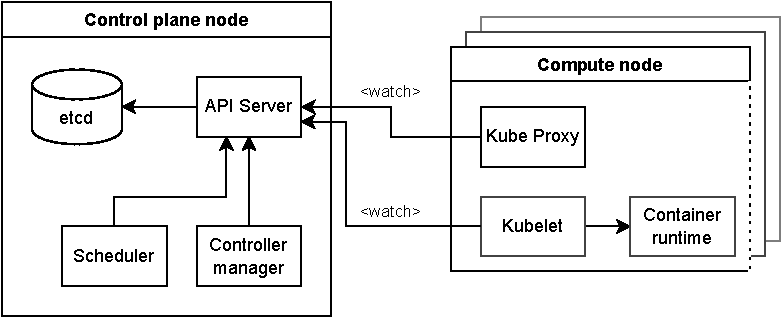
\includegraphics[width=.95\textwidth]{Figures/kubernetes-architecture.pdf}
	\caption{Core and compute services for Kubernetes\cite{Luksa.2018}}
	\label{fig.kubernetes-architecture}
\end{figure}

In the following paragraphs, the crucial services are described in detail. The so called \enquote{control plane node} or \enquote{master node} is the node where core services of \ac{K8s} are located. The underlying \ac{OS} must be Linux, because \ac{Windows} is not supported for the control plane. The other services can run on nodes (with any \ac{OS}) for executing the applications and perform computations (\enquote{compute node} or \enquote{worker node}). Since every service is a pod, they can have multiple replicas.

The services are controlled by the \ac{CLI} tools \enquote{kubectl} and \enquote{kubeadm}. While \enquote{kubectl} controls the deployment of services and application on the cluster, \enquote{kubeadm} is for setting up the cluster initially.
Furthermore, the tool \enquote{crictl} can be installed separately for the inspection of the local \ac{CRI} on a node. It allows insights into the containers and images, but also into locally running pods. Additionally, pods and containers can be managed using this tool.

\paragraph*{etcd}
The etcd\footnote{etcd: https://etcd.io/} database server is a key-value store designed for distributed systems\cite{Luksa.2018}. That means it could run with multiple replications and would still be able to keep a persistent storage synchronized across multiple instances. It contains the applied configuration of several cluster entities (e.g. User configurations, deployments, pod configurations).

\paragraph*{API server}
This is a RESTful web server that serves the \ac{K8s} \ac{API} via \ac{HTTP}\cite{Kubernetes.20221024}. It is the central joint between the services and establishes communication between users, external components and other core services. It makes the objects stored in etcd accessible through an Open \ac{API} specification\cite{Luksa.2018,OpenAPIInitiative.20230210} and allows observing changes on the entities. The \ac{CLI} tools \enquote{kubectl} and \enquote{kubeadm} both interact with the \ac{API} server.

\paragraph*{Kubelet} Kubelet is the service on the \ac{OS} level that maintains the pod life cycle and ensures the runtime of a container inside a pod. Furthermore, it manages the registration of the node to the control plane and reports its health and pod status to the \ac{API} server.

\paragraph*{Kube Proxy} The Kube-Proxy runs as a separate pod on every compute node. It maintains the connectivity between the services and pods\cite{Luksa.2018}. For a given \ac{IP} address and port combination it assures the connection to the corresponding pod. If multiple pods can offer a service, the proxy also acts as a load balancer\cite{Luksa.2018}.

\paragraph*{Scheduler} The scheduler is responsible for distributing services on the cluster and determining which node to choose during runtime. It reads conditions for scheduling (e.g. hardware resources, \ac{OS}, labels) from the \ac{API} server and decides which node matches the configuration\cite{Luksa.2018}.

\paragraph*{Controller manager} While the \ac{API}-Server is responsible for storing data in etcd and announcing changes to the clients, the Controller manager and its parts try to achieve a described target state\cite{Luksa.2018}. The controller manager consists of several controllers for replications, daemon sets, deployments, volumes, and so on.


\subsection{Pod life cycle}
\label{chap:design.life_cycle}
Similar to the underlying application container, Pods in \ac{K8s} have a ephemeral lifetime\cite{Kubernetes.20230217}. After creation on the cluster, a unique identifier is assigned before a pod gets scheduled to an available node\cite{Kubernetes.20230217}. The pod is kept alive until its termination or deletion\cite{Kubernetes.20230217}.
For distinguishing different kind of states of a pod life cycle, \ac{K8s} defines the pod states as described in \autoref{tbl:k8s-pod-states}.

\begin{table}[h!]
	\centering
	\begin{tabular}{|l | p{.65\textwidth}|} 
		\hline
		\bfseries State & \bfseries Description  \rule{-5pt}{2.6ex} \\
		\hline \rule{-3pt}{3ex}
		Pending & The pod has been set up, the container and pod is currently initialized. \\
		\hline
		Running & The pod is bound to a node, the container is running. \\
		\hline
		Succeeded & The container terminated with a zero exit code. \\ 
		\hline
		Failed & The container terminated with a non-zero exit code or was terminated by the system. \\ 
		\hline
		Unknown & The pod state could not be obtained. \\ 
		[1ex] 
		\hline
	\end{tabular}
	\caption{List of \ac{K8s} states during pod life cycle\cite{Kubernetes.20230217}.}
	\label{tbl:k8s-pod-states}
\end{table}

A terminated pod automatically gets restarted based on a configured restart policy. As the \ac{K8s} documentation states, \enquote{the kubelet restarts them [the containers of a pod] with an exponential back-off delay (10s, 20s, 40s, …), that is capped at five minutes}\cite{Kubernetes.20230217}. Furthermore, it is explained that the back-off time gets reset, once a container keeps running for 10 minutes\cite{Kubernetes.20230217}.


\subsection{Cluster networking}
Cluster networking is achieved using two components: The network plugin and the \ac{CNI}. Pods receive their own \ac{IP} address and can communicate with other pods. However, this is not a functionality which is achieved by \ac{K8s} directly. By using a \ac{CNI} the automated generation of network addresses and their inclusion is achieved when new containers are created or destroyed. It is crucial that pods share the same subnet across all the nodes in a cluster and \ac{NAT} is avoided\cite{Luksa.2018}.

Network plugins do implement the \ac{CNI}. They usually come with a manifest for a daemon set that introduces a network agent on all nodes inside the cluster to support the network communication.
For setting up the network interface, namespace and its \ac{IP} address, a dedicated container image is used. This is called the \enquote{pause container} image.

\paragraph*{Flannel}
Flannel\footnote{Flannel: https://github.com/flannel-io/flannel} was originally developed as part from Fedora CoreOS\footnote{CoreOS: https://getfedora.org/en/coreos}\cite{SuseRancherCommunity.20230212}. It works with various backends for transferring packets in the internal network. Two possible backends are \ac{VxLAN} and host gateway (\enquote{host-gw}). While \enquote{host-gw} needs an existing infrastructure and performs routing on the layer 3 network level, \ac{VxLAN} is more flexible and could also be used in cloud environments\cite{GitHubFlannel.io.20230212}. As shown in \autoref{fig:design.flannel-network}, \ac{VxLAN} is an overlay protocol and encapsulates layer 2 Ethernet frames within datagrams\cite{SuseRancherCommunity.20230212}. On top of the physical (underlay) network, the \ac{VxLAN} network provides their own \ac{IP} subnet. It is similar to regular VLAN and offers more than 4,096 network identifiers\cite{SuseRancherCommunity.20230212}. Thus, \ac{VxLAN} is a good choice for highly scalable systems.

\begin{figure}[h]
	\centering
	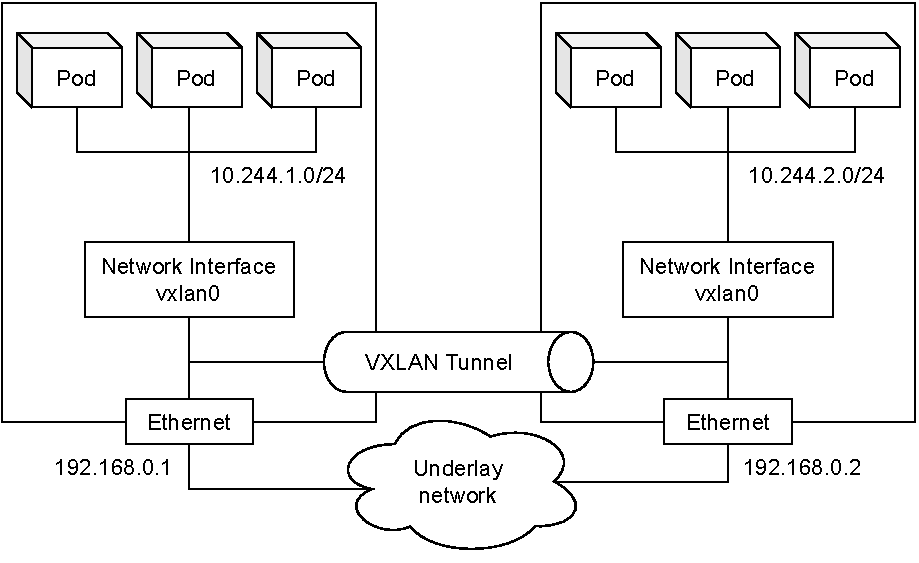
\includegraphics[width=.95\textwidth]{Figures/flannel-network.pdf}
	\caption{Flannel overlay network architecture for \ac{K8s}\cite{Schott.2019}. The pods have their own \ac{IP} address range and traffic gets routed through a \ac{VxLAN} tunnel.}
	\label{fig:design.flannel-network}
\end{figure}

Although the team behind \ac{K8s} does not recommend any specific network plugin, there are only a few common network plugins widely used. The amount of available \ac{CNI} plugins is even more reduced if the support for \ac{Windows} nodes is taken into account.

\paragraph*{Calico}
Compared to Flannel, Calico\footnote{Tigera's Calico: https://www.tigera.io/project-calico/} is stated to be more performative, flexible and powerful\cite{SuseRancherCommunity.20230212,Tigera.20230210}. Calico comes with a sophisticated access control system\cite{Tigera.20230210} and more configuration options. However, its advanced configuration makes it more complex to maintain long-term.

For this use case, Flannel is used as network plugin, since it is the more prominently used plugin used in the documentations for setting up \ac{K8s} with \ac{Windows} containers\cite{GitHubKubernetesSIGWindowsTools.20230213,Kubernetes.20220419}. Hence, support for this \ac{CNI} plugin in relation with \ac{Windows} containers is assumed to be larger than with Calico.




\section{Container environment}
The ecosystem around containerization defines terminology that needs to be looked at before going into details for \ac{K8s}. First of all, the container runtime defines the isolation layer between the physical host machine and the \ac{K8s} cluster. The \acf{CRI} defines the interface between \ac{K8s} and container runtime. Most of the container runtimes follow the design principles defined by the Open Container Initiative (OCI)\footnote{OCI: https://opencontainers.org/} for describing images and containers.
The container runtimes that are supported by \ac{K8s} are presented in this section.

While \ac{K8s} used to support Docker as their standard container runtime, they announced it to be deprecated in 2020, and finally removed the support in February 2022\cite{Kubernetes.2020, Kubernetes.2022}. The teams behind \ac{K8s} decided to drop the hard coded support for Docker and offer ContainerD instead.
However, the specification for ContainerD's \enquote{Containerfile} has only minor differences compared to Docker's \enquote{Dockerfile}. Thus, ContainerD files are fully compatible to docker files.

Some of the container runtimes offered by \ac{K8s} are not available for \ac{Windows} hosts. For example, Linux containers (LXC)\footnote{LXC: https://linuxcontainers.org/} use process groups, \acp{cgroup} and name spaces on the \ac{OS} level.
The \ac{CRI} from the Open Container Initiative (CRI-O)\footnote{CRI-O: https://cri-o.io/} is another alternative offered for \ac{K8s} on Linux systems. Since those are not available in \ac{Windows}, they are not further considered.


\subsection{Docker Container Runtime Interface}
The Docker \ac{CRI} (so called \enquote{Docker shim}) is using the internal mechanisms from Docker to run containers. The versions in Linux are using control group isolation.

For \ac{Windows}, there are two different isolation modes available. The first option is using the process isolation (so called \enquote{Host process isolation}) mode offered by ContainerD. It can be enabled by switching to \enquote{\ac{Windows} Containers}. It is the default mode for Windows Server systems.
However, older versions of Docker and Docker on Windows 10 and above have the opposite behavior\cite{RamosApolinario.2021}. On client versions of Windows, a dedicated hypervisor-isolated virtualization (so called \enquote{Hyper-V isolation}) is the default option\cite{RamosApolinario.2021}. This means, during the installation of Docker on \ac{Windows}, the underlying Windows container host creates a separate Hyper-V \ac{VM} to run container images. However, this is not a regular Hyper-V \ac{VM}\cite{RamosApolinario.2021}. Instead, it is a purpose-built \ac{VM}, often referred to as utility \ac{VM} or UVM that can't be managed directly and is fully controlled by the \ac{Windows} container runtime\cite{RamosApolinario.2021}. For networking, the internal mechanisms from Docker are used. All running containers are deployed inside the dedicated Hyper-V \ac{VM}. Therefore, this is a mixture of process isolation and full isolation using virtualization.

However, the hypervisor approach still has the disadvantage of using large resources for containers, even though they are running in one virtual machine. In addition, containers running in hypervisor isolation take longer to start up than those running in process isolation\cite{RamosApolinario.2021}.


\subsection{ContainerD}
ContainerD is a native version of a container runtime. Newer versions of Docker on Linux are running ContainerD as a basis for process isolation. On \ac{Windows}, ContainerD uses slim host process isolation.  The process isolation with ContainerD consists of multiple abstraction layers (shown in \autoref{fig.containerd-architecture}). Its back end contacts the containerd-shim which is maintaining an abstraction layer for communication for the underlying layers (depending on Linux and \ac{Windows}). Below that, \ac{Windows} offers a custom fork of the \ac{CLI} \textit{runc}, so called \textit{runhcs}\cite{Scooley.2022}. Using \textit{runc}, new containers can be created by running a simple command\cite{Scooley.2022}. The layer for \textit{runhcs} connects to the \ac{HCS} which is another abstraction layer of \ac{Windows} for providing a stable \ac{API} to the low level functionality of the \ac{OS}\cite{Microsoft.2017}. ContainerD does not come with any mechanisms for networking. Instead, this is in responsibility of the \ac{HCS}.

The developers of \ac{K8s} marked the Docker \ac{CRI} as deprecated in version v1.20\cite{Kubernetes.2020}. Since version v1.23 of \ac{K8s}, Docker was fully removed which lead to ContainerD being the only available \ac{CRI} for \ac{Windows} containers.

\begin{figure}[hb]
	\centering
	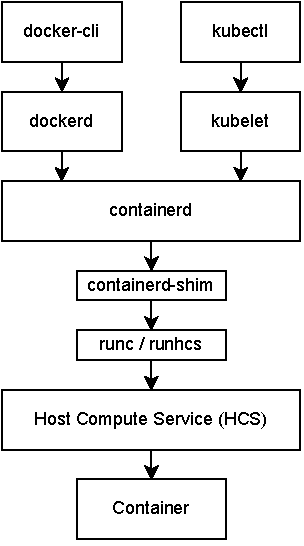
\includegraphics[width=0.4\textwidth]{Figures/containerd-architecture.pdf}
	\caption{Abstraction layers for ContainerD on Windows. The image shows the technology stack from the Docker and \ac{K8s} command line to the Container layer.\cite{Scooley.2022}}
	\label{fig.containerd-architecture}
\end{figure}

There are two \ac{CLI} tools that work with ContainerD. The tool \enquote{ctr} is the low level \ac{CLI} tool that is shipped with ContainerD.  \enquote{nerdctl} is a tool that is similar to the Docker \ac{CLI}  and supports the same set of commands and options as Docker. Compared to \enquote{ctr}, however, \enquote{nerdctl} is more feature-rich.



Currently, container networking with ContainerD is not well-established on \ac{Windows}~\cite{GitHub.20230202,GitHub.20230202b,Github.2022_258,GitHub.20230202c} even though the docker runtime is already removed in current versions of \ac{K8s}~\cite{Kubernetes.2020}. However, these are the only two working container backends for \ac{Windows} containers. Therefore ContainerD as container backend was chosen.



\section{Container Image}
There are container images for each process of the system architecture, each of them having their own Containerfile definition with different command line arguments and environment variables.
The container image and its base image is further explained in this section.

\subsection{Base image}
The container images to use for running the OpenTwin processes need to run a \ac{Windows} base image. Beside the full \ac{Windows} images, Microsoft offers the more common images \enquote{\ac{Windows} Server Core} and \enquote{\ac{Windows} Nanoserver}\cite{MattbriggsMicrosoft.20230214}. They significantly differ in the download size, their on-disk footprint and the features supported\cite{MattbriggsMicrosoft.20230214}. As Microsoft states, \enquote{Nanoserver was built to provide just enough \ac{API} surface to run apps that have a dependency on .NET core or other modern open source frameworks. PowerShell, Windows Management Instrumentation, and the \ac{Windows} servicing stack are absent from the Nanoserver image}\cite{MattbriggsMicrosoft.20230214}.

The design of containerization of \ac{OT} envisages the usage of \enquote{Server Core} as base image. Even though the \enquote{Server Core} image is not the smallest base image, it provides full functionality for the required technologies for the current use case.

% Warum dieses \ac{Windows} image?
% \ac{Windows} Server Core and Nanoserver are the most common base images to target. The key difference between these images is that Nanoserver has a significantly smaller \ac{API} surface. PowerShell, WMI, and the \ac{Windows} servicing stack are absent from the Nanoserver image.
% Nanoserver was built to provide just enough \ac{API} surface to run apps that have a dependency on .NET core or other modern open source frameworks. As a tradeoff to the smaller \ac{API} surface, the Nanoserver image has a significantly smaller on-disk footprint than the rest of the \ac{Windows} base images. Keep in mind that you can always add layers on top of Nano Server as you see fit. For an example of this check out the .NET Core Nano Server Dockerfile.
% Quelle: https://learn.microsoft.com/en-us/virtualization/\ac{Windows}containers/manage-containers/container-base-images

\subsection{Custom image}
On top of the base image, customizations and the actual application are applied. The binary files are included in the container image and added during build. The common \acp{CRI} only forward the output of processes with process id 1 to the host machine. Furthermore, this is also the only process the  \ac{CRI} is waiting for, to keep the container alive. Thus, instead of using the provided batch files to start the application services, the OpenTwin process is called directly with the appropriate command line arguments as command for the container.
Therefore, the environment variables needs to be set up as part of the container file.
The root certificate (certificate authority) is passed as file mount into the container later on.

\vspace{2em}
\section{Target architecture}
The application is distributed on multiple hosts. \ac{K8s} supports application rollouts only as container images. To be able to distribute the services on a cluster management tool a containerization of the application is necessary.
Each service must be operated on the cluster to profit from the features which \ac{K8s} offers. For example, it should be possible to offer multiple replications of services - with the compute services included. This is the only way to ensure that the application can be delivered reliably. 
However, for testing the feasibility it is sufficient to deploy only the main services as a first step. This involves \ac{GSS}, \ac{LSS} and \ac{AUTH}. Subsequently, the \ac{LSS} spawns the compute services as sub processes inside the same container. In order to communicate with the \ac{UI} front end, the connection between the external network and the relay service has to be ensured.

The MongoDB server is not required to run on \ac{Windows}. Because setting it up on Linux is easier and better supported, a dedicated Linux node for running the MongoDB server is preferred. Furthermore, automation for a MongoDB container image on \ac{Windows} is currently unsupported, because of an design limitation in Windows containers\cite{GitHub.20230317}. The \ac{OT} services, however, have to run on \ac{Windows} and are therefore deployed on a \ac{Windows} node.

The encrypted communication between services has to be ensured. As a consequence, the certificates need to be accessible for each service. The certificate files shall be published on the container file system using file mounts. This increases flexibility, because files can be easily swapped out and generated for each service outside the container. Certificate files then have to be created during pod creation.
However, as a first step, the certificates are generated as part of the image build process to keep the automation simpler.



